\chapter{Software Requirements Specification}

	
	\begin{flushright}
		\rule{16cm}{5pt}\vskip1cm
		\begin{bfseries}
			\Huge{}\\
			\vspace{0.5cm}
			for\\
			\vspace{1.5cm}
			Object Detection using Google Earth \\
			\vspace{1.5cm}
			\LARGE{Version 1.2 \myversion}\\
			\vspace{1.5cm}
			Prepared by : SujayKumar Reddy M (20BDS0294)\\
			\vspace{1.5cm}
			Sahaaya Arul Mary S.A
		\end{bfseries}
	\end{flushright}
	
	
	\section{Introduction}
	
	\subsection{Purpose}
	The usage of \textbf{Google Earth} and \textbf{Google Street View} is not very habitated by the users. In fact we can do many things for example Detecting Rooftops, Detection of more Heavy Vehicles to reduce the Pollution, in these applications this  product is specifically intended for. As when the Vehicle is in transit we cannot  track the vehicle in google earth because google earth is a satelite imagery where we cannot watch live changes.According to my research the google earth satellite imagery updates the images for every 1 to 3 years and NASA's Livestat project updates for every 16 days. This application is very much useful for drones to detect the roof-tops and all other Static Objects.My tool will be an interface for the research community for analyzing the vegetation in a particular area within a period of 2-3 years and Rooftop Detection for the drones to deploy a model and other various static applications. My tool will be an interface for all the entities which are available and they can use this to detect the produced Objects and this is the main concept of my model/tool.
	
	% This is very much difficult to maintain all the data of a course as a hard copy. Any data can be changed, deleted, added at any time. Such as - A new teacher can be assigned for a course, he also can be changed ; And so many student are getting admitted every semester. So, "IICT WEBSITE" is the solution. "IICT WEBSITE" is a official website based on marking and resulting system of IICT authorized. The main concept of "IICT WEBSITE" is to devitalized PGD, MIT courses, their students and teachers data maintenance. 
	%
	
	
	\section{Document Conventions}
	\begin{tabular}{ p{4.5cm} p{8cm} }
		
		
		GEE         &Its an API Service by Google named as Google Earth Engine.\\\\
		GSV         &Google Street View is an API Service Provided by the GEE and it mainly concentrates on Street Photography useful for AR/VR Apps \\\\
		Static Objects  &The Object which cannot be changed over 2-3 years of time like Buildings, farms and Vegetation within a particular reach.\\\\
		Tflite		&An Tensorflow Model which is used to Generate the Supervised Learning Approach for the Static Object Detection\\\\
				
		
		
	\end{tabular}
	
	
	\section{Intended Audience and Reading Suggestions}
	This Software Requirement Specification is for Myself for the future reference, Professor and testers.This SRS is done according to the template given by the Professor. Issues List is provided at the end of the document at Appendix C. Further, the discussion will provide all the internal, external, functional, and also non-functional information about "Object Detection from Google Earth Images". 
	
	
	
	
	
	
	
	
	\section{Project Scope}
	The Major Stakeholders are the ... 
	\begin{enumerate}
		\item User
		\item GEE
		\item Object Identification
		\item Time
		\item Tracking 
	\end{enumerate}
	GEE will take care with the communication of the satellites and takes in the data of satellite image processing. We will only consider that processed image as the input to our model or tool. The GEE API Service will give us an API Services where we can navigate for a zommed in image to process the image carefully. The Service would be connected with our System which will detect the Objects and track the motion of the detected object.
	\newline
	Object Identification is an Machine Learning Model which detects the objects by Open CV2 it marks the object and classifies as an provided class label.
	\newline
	The User communicates with the GEE Service through our interface and gives us the starting co-ordinates and starting image to identify.
	\newline
	The Time is important because we are considering the static imagery of the Google Earth Engine. We need the images which are useful for real time data by using various sensors but the dataset which we use to train our data.
	\newline
	\begin{center}
		\begin{figure}
			\centering
			\includegraphics[scale=0.32]{images/2.png}
			\caption{Entire work-flow}
			\label{}
		\end{figure}
	\end{center}
	
	Figure 1.1 (Entire work-flow) is the overview of the project. Connection of all the entities are dependable to each others.  This gives the simple idea about the functional activities of the project. 
	\newline
	Google Earth Engine will be a static input for our web application because the model which we trained for.
	\newline
	So, every entity is vary much interactive with each other.
	
	The project scope for Object Detection from Google Earth Images would typically include the following:
	
	\begin{enumerate}
		\item Object Detection Algorithm: Develop a computer vision algorithm to detect objects in Google Earth images using techniques such as convolutional neural networks (CNNs), region-based convolutional neural networks (R-CNNs), and You Only Look Once (YOLO) algorithms.
		\item Image Dataset: Create or obtain a dataset of Google Earth images for training and testing the object detection algorithm. The dataset should include a variety of different objects in different environments and under different conditions.
		\item Model Training: Train the object detection algorithm using the image dataset. This will involve adjusting the parameters and architecture of the model until it can accurately detect objects in the images.
		\item Model Deployment: Integrate the trained object detection model into an application that can be used to process Google Earth images and detect objects within them.
		\item User Interface: Develop a user interface that allows users to select an image from Google Earth, process it with the object detection model, and view the results. The interface should be intuitive and easy to use.
		\item Performance Evaluation: Evaluate the performance of the object detection model by comparing its results to a ground truth dataset. This will involve measuring metrics such as precision, recall, and accuracy.
		\item Optimization: Optimize the performance of the object detection model by making changes to the algorithm, dataset, or other aspects of the system as necessary.
	\end{enumerate}
	
	
	% \section{References}
	% \url{}{}
	
	
	
	
	
	
	
	
	
	
	
	
	
	
	
	
	
	\section{Overall Description}
	
	\subsection{Product Perspective}
	Google earth is a large system and My Tool integrates into this particular API Services for providing various analysis of geo-spatial data. Main goal of this project is to minimize the workflow of using drones to calculate the static data instead we can use our tool to Identify the static objects for data analysis.
	
	
	
	
	
	
	
	
	
	\subsection{User Classes and Characteristics}
	This Object Detection has basically 2 types of users. 
	\begin{itemize}
		\item Researchers
		\item Business Entitites 
	\end{itemize}
	The Researchers working on SOLAR Energy they have the very useful application to know how much area does the each village has so we can implement it by comparatively.\\\\
	The Business Entities like Amazon can use the models to detect the rooftops to deliver the packages for per user.
	% \begin{figure}
		%     \centering
		%     \includegraphics[width=10cm]{2.JPG}
		%     \caption{type of users}
		%     \label{fig:type of users}
		% \end{figure}
	
	\subsection{Product Functions}
	The Product should be able to detect the rooftops for the drones in-order to land the package for asset management services. If the Object is the Farming Lands then the Drone would find the optimal point where all the agriculture sensors would be able to communicate within the distance.
	
	Before using the main function of the software result process, users have to be registered. 
	\newline
	The Products primary source is the Machine Learning model. Result is the main feature of all. It contains the Object which is marked by the Open CV2.
	
	\subsection{Operating Environment}
	The website will be operate in any Operating Environment - Mac, Windows, Linux etc. 
	
	\subsection{Design and Implementation Constraints}
	As the ML model is the primary source we consider that as a Design.
	\begin{itemize}
		\item From the Unprocessed Image from the GE.
		\item Supervised Learning Techniques.
		\item Class Labels and Unsupervised Learning Techniques.\\
	\end{itemize}


	From the GE Image we need to detect the static objects and find a suitable environment with color grading which would provide us an Undefined colored so, it acn be easily seen by the Sensors or Microcontrollers in the Drones.\\
	
	Every Image would happen to work with utmost accuracy to detect the static images.\\\\
	
	Design and implementation constraints for object detection from Google Earth can vary depending on the specific use case and requirements. However, some common constraints and considerations are:

	

	

	\begin{itemize}
		\item Image Quality: The quality and resolution of the satellite images in Google Earth can have a significant impact on the accuracy and reliability of object detection. Poor quality images with low resolution, or images that are obstructed by clouds or other factors, can make it difficult to accurately detect objects.
		\item Object Variability: The variability of objects in satellite images can also impact the accuracy and reliability of object detection. Objects may vary in size, shape, orientation, and appearance, which can make it challenging to train object detection algorithms to recognize them.
		\item Computational Resources: Object detection can be computationally intensive, and large amounts of data need to be processed in real-time to ensure fast and accurate results. It is important to carefully consider the computational resources required to run the object detection algorithm, as well as the hardware and software infrastructure required to support it.
		\item Data Privacy and Security: Google Earth images may contain sensitive information that needs to be protected, and it is important to ensure that the object detection algorithm is designed and implemented in a way that protects this information.
		\item Data Storage and Management: The amount of data generated by object detection from Google Earth images can be large, and it is important to have a robust and scalable data storage and management system in place to handle this data.
	\end{itemize}

These are some of the key design and implementation constraints for object detection from Google Earth. However, there may be additional constraints and considerations that are specific to your use case and requirements.
	
	
	
	
	
	
	
	
	
	
	
	
	
	
	\section{System Features}
	
	
	
	\subsection{Functional Requirements}
	\begin{enumerate}
		\item The object detection software should be able to process images from Google Earth and extract relevant information for object detection. This may involve implementing algorithms for image pre-processing, such as image resizing, and image normalization.
		\item The object detection software should be able to detect objects of interest in the images, such as buildings, vehicles, and roadways. This may involve implementing object detection algorithms, such as deep learning-based object detection, and training the algorithms on annotated image data.
		\item The object detection software should be able to classify the objects detected in the images into relevant categories, such as type of building, type of vehicle, or type of roadway. This may involve implementing object classification algorithms and training the algorithms on annotated image data.
		\item The object detection software should be able to locate the objects in the images and provide the coordinates of the objects. This may involve implementing object localization algorithms, such as bounding box regression, and training the algorithms on annotated image data.
		\item The object detection software should be able to generate outputs, such as annotated images or data reports, that provide information about the objects detected in the images. This may involve implementing output generation algorithms and user interfaces for visualizing the outputs.
		\item The object detection software should provide user interfaces for interacting with the software, such as uploading images, configuring the object detection algorithms, and viewing the outputs. This may involve implementing graphical user interfaces, command line interfaces, or application programming interfaces (APIs) for integrating the object detection software with other software systems.
	\end{enumerate}
	
	
	
	
	
	
	
	\section{External Interface Requirements}
	TensorFlow Lite (TFLite) is a lightweight version of TensorFlow, designed to run on resource-constrained devices such as mobile phones and embedded systems. The TFLite object detection model can be integrated into various external user interfaces to provide object detection capabilities to end users. Some common external user interfaces for TFLite object detection models are:
	\begin{enumerate}
		\item Mobile Applications
		\item Web Applications
		\item Embedded Systems.
		\item Robotics
	\end{enumerate}
These are some of the external user interfaces that TFLite object detection models can be integrated with. The specific user interface that you choose will depend on your use case and requirements. It is important to carefully consider the requirements of your application and the resources available on your target device when selecting an external user interface for your TFLite object detection model.

\subsection{Software Interfaces}
\begin{enumerate}
	\item Mobile SDKs: TFLite object detection models can be integrated into mobile software development kits (SDKs), allowing developers to build mobile applications that perform object detection on mobile devices.
	\item Web API: TFLite object detection models can be deployed as web APIs, allowing object detection to be performed over the internet. This can be useful for building cloud-based object detection systems that can be accessed by a variety of clients, such as mobile applications, web applications, and desktop applications.
	\item Robotics API: TFLite object detection models can also be integrated into robotics APIs to provide object detection capabilities for autonomous robots.
	\item Embedded API: TFLite object detection models can be integrated into embedded APIs, allowing developers to build custom embedded systems that perform object detection.
	 
\end{enumerate}

\subsection{Hardware Interfaces}
The Google Earth API can be integrated with various hardware interfaces to provide mapping and visualization capabilities to end users. Some common hardware interfaces for the Google Earth API are:
\begin{enumerate}
\item Web Browsers: The Google Earth API can be integrated into web browsers to provide interactive mapping and visualization capabilities to end users. This allows users to access Google Earth in their web browsers and interact with maps and satellite imagery.
\item Embedded Systems: The Google Earth API can be integrated into embedded systems, such as GPS devices and in-vehicle navigation systems, to provide mapping and visualization capabilities in these environments.
\item Robotics Hardware: The Google Earth API can also be integrated into robotics hardware, such as autonomous robots, to provide mapping and navigation capabilities for these systems.
	
\end{enumerate}
These are some of the hardware interfaces that the Google Earth API can be integrated with. The specific hardware interface that you choose will depend on your use case and requirements. It is important to carefully consider the requirements of your application and the resources available on your target device when selecting a hardware interface for the Google Earth API.


	\section{Other Nonfunctional Requirements}
	
	\subsection{Performance Requirements}
	The performance requirements for object detection from Google Earth images will depend on a number of factors, including the size of the images, the complexity of the objects being detected, the desired accuracy and speed of the object detection process, and the resources available on the hardware platform where the object detection is being performed. Some of the key performance requirements for object detection from Google Earth images include:
	\begin{enumerate}
		\item Computational Power: Object detection algorithms can be computationally intensive, and therefore a powerful processing platform is necessary to perform object detection in real-time. This may involve using high-performance CPUs, GPUs, or other specialized hardware such as Tensor Processing Units (TPUs).
		\item Memory: Object detection algorithms require large amounts of memory to store the image data and intermediate results of the object detection process. Therefore, the hardware platform should have sufficient memory to support the object detection process.
		\item Network Bandwidth: If the object detection is being performed in a cloud environment, the network bandwidth between the cloud and the client device may also be a factor in the performance of the object detection process.
		\item Latency: The latency of the object detection process is an important factor in the overall performance of the system. Latency refers to the time it takes for an object detection request to be processed and the results to be returned to the client. Low latency is important for real-time applications where the results of the object detection process need to be available immediately.
		\item Accuracy: The accuracy of the object detection process is also a critical factor in the overall performance of the system. High accuracy is important for applications where the object detection results are used to make important decisions, such as in autonomous vehicles or surveillance systems. 
	\end{enumerate}
These are some of the key performance requirements for object detection from Google Earth images. The specific performance requirements for your application will depend on the details of your use case and the desired outcomes. It is important to carefully consider the performance requirements of your application and the resources available on your hardware platform when designing and implementing an object detection system from Google Earth images.
	
	\subsection{Security Requirements}
	Security is an important consideration in any application that involves processing and storing sensitive information, including object detection from Google Earth images. Some of the key security requirements for object detection from Google Earth images include:
	
	\begin{enumerate}
		\item Data Privacy: The privacy of the image data being processed and stored must be protected. This may involve encrypting the image data and ensuring that it is only accessible by authorized individuals.
		\item Data Integrity: The integrity of the image data must be protected to prevent unauthorized changes to the data. This may involve implementing data integrity checks and audit trails to detect any unauthorized changes to the data.
		\item Access Control: Access to the image data and the object detection results must be controlled to ensure that only authorized individuals have access to the data. This may involve implementing user authentication and authorization mechanisms, such as usernames and passwords, to control access to the data.
		\item Network Security: The network over which the image data is transmitted and the object detection results are returned must be secure to prevent unauthorized access to the data. This may involve implementing encryption algorithms, such as SSL/TLS, to secure the data transmission.
		\item Physical Security: The hardware platform where the object detection is performed must be physically secured to prevent unauthorized access to the image data and the object detection results. This may involve implementing physical security measures, such as security cameras, access controls, and secure data storage facilities.
		
	\end{enumerate}
These are some of the key security requirements for object detection from Google Earth images. The specific security requirements for your application will depend on the sensitivity of the image data and the desired level of security. It is important to carefully consider the security requirements of your application and to implement appropriate security measures to protect the image data and the object detection results.

\subsection{Software Quality Attributes}
		Software quality attributes are characteristics of software that are important to ensure that the software is fit for its intended use. In the context of object detection from Google Earth images, some of the key software quality attributes include:
		\begin{enumerate}
			\item Usability: The object detection software should be easy to use and understand for the end-users. This may involve providing clear and concise user interfaces, user-friendly error messages, and intuitive navigation.
			\item Reliability: The object detection software should be reliable and should perform its intended functions accurately and consistently. This may involve implementing robust error handling mechanisms, redundant components, and regular software testing.
			\item Performance: The object detection software should perform efficiently and quickly, especially for real-time applications. This may involve optimizing the algorithms for the hardware platform, reducing latency, and improving computational performance.
			\item Scalability: The object detection software should be able to handle increasing volumes of image data and users without degradation in performance. This may involve implementing scalable algorithms and architectures, load balancing, and distributed computing.
			\item Maintainability: The object detection software should be maintainable, so that it can be updated and improved over time. This may involve writing clear and well-documented code, using modular design patterns, and following software development best practices.
		\end{enumerate}
	
	

	
	
